\chapter{Tracking Module}
\label{cha:track}

Visual tracking is the process of determining the position of a target
in a sequence of images. The localization of the target in the image
can be useful in several applications such as robotics,
video-surveillance, and many others.

In \rox{}, the selection of the target can be done by the user manually
with a selection of an appropriate Region Of Interest (ROI) in the
reference image. If the user has already defined such an ROI, \rox{} allows to identify a given image model in the current image. The
identification module is also used to re-identify the target if the tracking is
lost (for example if the ROI is occluded or out of the image).

The Tracking module contains the following sub-modules:

\begin{description}
  \item[Tracking Parameters]~: module with structures and methods for handling the tracking parameters~;

  \item[Tracking]~: module with structures and methods for tracking 2D objects~;

\end{description}

\section{Tracking Parameters}
\label{sec:tracking_params}

\subsection{The Rox\_Tracking\_Params object}
\label{sse:tracking_params_object}

The object \lstinline$Rox_Tracking_Params$ contains several
parameters that can be used to define the visual tracking.
The basic shape for an area of interest is a rectangle. However,
the user can also define a region of interest inside a polygon or create
a customized area with image masks. The most important parameters are the following:

\begin{itemize}
\item Iteration number
\item Tracking precision
\item Prediction area
\item Use of Kalman filter
\item Score threshold  
\end{itemize}

The tracking parameters are stored in a \lstinline$Rox_Tracking_Params_Struct$ structure. A \lstinline$Rox_Tracking_Params$ object is opaque and can be accessed using the pointer to a \lstinline$Rox_Tracking_Params_Struct$ structure: 
\begin{lstlisting}
typedef struct Rox_Tracking_Params_Struct* Rox_Tracking_Params;
\end{lstlisting}

\subsection{Creating/Deleting a Rox\_Tracking\_Params object}
\label{sse:tracking_params_creating}

\rox{} provides functions to create / delete the Rox\_Tracking\_Params structure~:

\begin{lstlisting}
Rox_Tracking_Params rox_tracking_params_new(Rox_Void);
\end{lstlisting}
The \lstinline$rox_tracking_params_new$ function allocates memory for the structure, 
sets parameters with default values (\lstinline$miter = 10$, \lstinline$mprec =  0$, \lstinline$mpred = 16$, \lstinline$score_thresh = 0.89$, \lstinline$kalman = ROX_TRUE$, \lstinline$auto_update = ROX_FALSE$, \lstinline$light = ROX_FALSE$) and returns a pointer on the newly created structure.\\

\begin{lstlisting}
Rox_Tracking_Params rox_tracking_params_new_readfile (Rox_File filename);
\end{lstlisting}
The \lstinline$rox_tracking_params_new_readfile$ function allocates memory for the structure,
reads the `filename' \lstinline$Rox_File$ and sets parameters with read values. A pointer on the newly created patch is returned by this function.\\

\begin{lstlisting}
Rox_Void rox_tracking_params_del(Rox_Tracking_Params Params);
\end{lstlisting}
The \lstinline$rox_tracking_params_del$ function deallocates memory for a parameter structure. It
is necessary to call this function when the structure is not used anymore or before overwriting it.

\subsection{The main functions related to the object Rox\_Tracking\_Params}
\label{sse:tracking_params_functions}

The tracking algorithm has four important parameters set at the parameters structure
initialization~: `miter', `mprec', `mpred', `mtime'. Functions are provided to set these parameters~:

\begin{itemize}
%  \item \lstinline$rox_tracking_params_set_mtime$~: Sets mtime parameter~;
  \item \lstinline$rox_tracking_params_set_miter$~: Sets miter parameter~;
  \item \lstinline$rox_tracking_params_set_mprec$~: Sets mprec parameter~;
  \item \lstinline$rox_tracking_params_set_mpred$~: Sets mpred parameter~;
\end{itemize}

Setting a parameter with a strictly negative value (typically -1) will
leave it unchanged. \\

%{\bf Warning :} If a null value is set for `miter' and / or `mprec', no iteration at
%all of the ESM algorithm will be performed ! In this case, if `mpred' is not null, a tracking
%only based on the prediction will be performed, else there will be no tracking
%at all. \\

It is not mandatory to use the same parameters during the whole
sequence. For example, a part of the sequence may need a prediction
phase and few iterations because of a known high translation, but we
would rather use more iterations without prediction for the rest of
the sequence. Thus, some parameters can also be changed in runtime using
function described in \ref{sss:track2D_setparam}.

\subsubsection{Setting the parameters for tracking objects with changing shape or appearence}
\label{sss:tracking_params_examples}

In some applications, as for example the visual tracking of targets
with changing shape or appearence such as pedestrians, it is more
stable to freeze some degrees of freedoms of the homography. The
function
\lstinline$rox_tracking_params_set_tracking_model$ allows the user to
track such targets using the following transformation:
\[
{\bf H} = \left[ \begin{array}{ccc} homog[0] & 0 & homog[2] \\ 0 & homog[4] & homog[5] \\  0 & 0 & homog[8] \end{array} \right]
\]
which provides not only the translation of the template in the image but also its anisotropic scaling (see Figure~\ref{scale}).

\begin{lstlisting}
enum Rox_Tracking_Model_Enum {Rox_Tracking_Model_tu, 
			      Rox_Tracking_Model_tv,
			      Rox_Tracking_Model_tu_tv_s, 
			      Rox_Tracking_Model_tu_tv_su_sv, 
			      Rox_Tracking_Model_tu_tv_s_r, 
			      Rox_Tracking_Model_SL3 };
\end{lstlisting}

\begin{itemize}
\item \lstinline$Rox_Tracking_Model_tu$ with this model the target motion is supposed to be a translation along the u axis;
\item \lstinline$Rox_Tracking_Model_tv$ with this model the target motion is supposed to be a translation along the v axis;
\item \lstinline$Rox_Tracking_Model_tu_tv_s$ with this model the target motion is supposed to be a translation and an isotropic change of scale;
\item \lstinline$Rox_Tracking_Model_tu_tv_su_sv$ with this model the target motion is supposed to be a translation and an anisotropic change of scale;
\item \lstinline$Rox_Tracking_Model_tu_tv_s_r$ with this model the target motion is supposed to be a translation, an isotropic change of scale and a rotation around the optical axis;
\item \lstinline$Rox_Tracking_Model_SL3$ with this model the target motion is supposed to be a homographic transformation;
\end{itemize}

\begin{figure}[htbp] 
\begin{center}
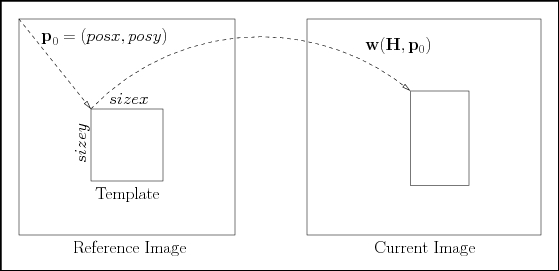
\includegraphics[width=1.0\textwidth]{tracking/figures/scale}
\caption{Translation and scaling of the reference template.}
\label{scale}
\end{center}
\end{figure}

In several applications, when tracking deformable objects it is better to fix the model to \lstinline$Rox_Tracking_Model_tu_tv_s$ or \lstinline$Rox_Tracking_Model_tu_tv_su_sv$.

% \subsubsection{Setting the parameters for tracking in the whole image or for target identification}
% \label{sss:tracking_params_ident}
% When the target make very large displacement in the image, it is sometimes necessary to search the target in the whole image. The same problem can arise when the target is lost, occluded or out of the image and the it comes back in the camera field of view. \rox{} allows the user to identify the target by choosing several identification methods using the following function:
% \begin{lstlisting}
% rox_tracking_params_set_ident(Rox_Tracking_Params P, Rox_Sint ident)
% \end{lstlisting}
% Setting ident to 0 will disable the research. The methods 1 and 2 are more robust but slower. The methods 2 and 4 are faster but the identification success rate is lower.

% The research time in the whole image may be a time consuming step. Thus it is possible to reduce the computation time by setting a parameters that tell to \rox{} to reduce the size of the image before the research. The use can use the following function:
% \begin{lstlisting}
% rox_tracking_params_set_ident_full_image(Rox_Tracking_Params P, Rox_Bool ident_full_image)
% \end{lstlisting}


\section{Tracking}
\label{sec:tracking}


\subsection{The Rox\_Tracking object}
\label{sse:tracking_object}

A \lstinline$Rox_Tracking$ object can be defined using the pointer to a \lstinline$Rox_Tracking_Structure$:
\begin{lstlisting}
typedef struct Rox_Tracking_Struct* Rox_Tracking;
\end{lstlisting}

\subsection{Creating/Deleting a Rox\_Tracking object}
\label{sss:track2d_initializing}

Functions are provided to allocate and deallocate a \lstinline$Rox_Tracking$ structure~:
\begin{lstlisting}
Rox_Tracking rox_tracking_new(Rox_Tracking_Params P, Rox_Camera C);
\end{lstlisting}
The \lstinline$rox_tracking_new$ function allocates memory for the structure of the track object, according to
the `P' parameters and returns a pointer on the newly created structure. \\

% \begin{lstlisting}
% Rox_Tracking rox_tracking_new_rect (
% 	Rox_Image 	I, 
% 	Rox_Window 	W,
% 	Rox_Uint 	miter, 
% 	Rox_Uint 	mprec, 
% 	Rox_Uint 	mpred);
% \end{lstlisting}
% The \lstinline$rox_tracking_new_rect$ function allocates memory for polygon and initialize it according to parameter `W' 
% and returns a pointer on the newly created structure. \\

% \begin{lstlisting}
% Rox_Tracking rox_tracking_new_poly (	
% 	Rox_Image 	I, 
% 	Rox_Sint 	*pts, 
% 	Rox_Sint 	nb_pts, 
% 	Rox_Uint 	miter, 
% 	Rox_Uint 	mprec, 
% 	Rox_Uint 	mpred);
% \end{lstlisting}

% The \lstinline$rox_tracking_new_rect$ function allocates memory for polygon and initialize it according to parameter `nb\_pts' 
% and returns a pointer on the newly created structure.

%%%%%%%%%%%%%%%%%%%%%%%%%% User: Odometry and Tracking %%%%%%%%%%%%%%%%%%%%%%%%%%%%%%%%%%%%
% \ifthenelse{\boolean{USER_TRACKING} \or \boolean{USER_ODOMETRY}}
% {
% The variables {\tt miter} and {\tt mprec} shall be initialized by the
% user. The variable {\tt miter} contains the maximum number of
% iterations for the minimization algorithm and the {\tt mprec} number
% corresponds to the precision of the tracking result. Both numbers
% should be always bigger than (or equal to) {\tt 1}. The user sets
% these numbers depending on the frame-rate of the acquisition of the
% images, on the power of the computer used and on the size of the
% template to track. For an acquisition frame-rate around 30 fps and a
% processor equivalent to Pentium IV 2GHz, setting {\tt miter = 10} and
% {\tt mprec = 3} gives good results when tracking a {\tt
%   (150}$\times${\tt 150)} template.
% The parameter  {\tt mpred} is a positive integer defining a search area around the template. 
% Setting the value of {\tt mpred} big allows handle important inter-frame displacements (the displacements of the target in two consecutive images can be big). 
% However, this slows down the visual tracking. A value of {\tt mpred} equal to {\tt 8} is a good compromise between speed and robustness. \\
% }
%%%%%%%%%%%%%%%%%%%%%%%%%% End of User: Odometry and Tracking %%%%%%%%%%%%%%%%%%%%%%%%%%%%%%%%%%%%
% \noindent These functions allocate memory for the \lstinline$Rox_Tracking$ structure and its field, 
% build image pyramid(s) from the reference patch / list of references patches and set
% the initial homography to the $3 \times 3$ identity matrix. If one does not want
% to build and use image pyramids, just set mprec to zero.\\

\begin{lstlisting}
Rox_Void rox_tracking_del(Rox_Tracking T);
\end{lstlisting}
The \lstinline$rox_tracking_del$ function deallocates memory for a \lstinline$Rox_Tracking$ structure. 
It is necessary to call this function when the structure is not used any more or before overwriting it. \\

The \lstinline$Rox_Tracking$ structure is opaque, i.e. its internal fields are hidden
and cannot be accessed directly by the user. A
consequence is that the user can only declare and manipulate pointer on this
structure, and never the structure itself, as the size of the structure 
is unknown to the user.\\

% In case of list of several patches, all of them shall be coplanar. Each can be
% generated using the `new' tool described above. The different patches are not
% tracked individually~: they are all unified in a unique system to solve. Thus,
% there is only one resulting homography, which correspond to the motion of the
% plane they belong to. \\

In order to track individually several patches, the user can declare and create
several \lstinline$Rox_Tracking$ structures and perform the algorithm on each of
them. The patches may also belong to different planes.\\

% \pagebreak %Specific

\subsection{The main functions related to the object Rox\_Tracking}
\label{sss:tracking_methods}

Once the \lstinline$Rox_Tracking$ is allocated and initialized, it is possible to:
\begin{itemize}
  \item Predict large motion
  \item Perform tracking pf planar objects
  \item Change tracking parameters
  \item Set the mask to track a generic template
  \item Measure the quality of the tracking
\end{itemize}


\subsubsection{Prediction}
\label{sse:prediction}

%\paragraph{Motivation}
%\label{par:prediction-motivation}

When a huge displacement occurs
between two frames of a sequence, due either to a fast motion or to a
low frame rate, the tracked object can get ``lost''.\\

In order to handle large displacement,
a phase of prediction can be introduced prior to the tracking
algorithm. It has to find the tracked object in a search window to
determine a translation applied to the current homography matrix and
then some iterations of the tracking algorithm can locally refine
the displacement.\\

The search window is set by the `mpred' parameter of the tracking
structure, which defines the number of pixels around the current
position of the tracked object.\\

As the prediction may be an expensive process, it is possible to skip it by
setting the `mpred' tracking parameter to zero.

\subsubsection{Perform tracking of planar objects}
\label{sss:tracking_perform}

To perform the tracking we call the \lstinline$rox_tracking_make$ function with the \lstinline$Rox_Tracking$ structure 
and the camera containing the image where to perform the tracking as parameters. This function shall be called for each image of the sequence. 

The resulting homography can be retrieved using the function:
\begin{lstlisting}
rox_tracking_get_matsl3_copy
\end{lstlisting}

which
returns a pointer on a $3 \times 3$ matrix. This homography can be used for example to draw a black box around the tracked
object in the image sequence, using the function:
\begin{lstlisting}
rox_image_draw_target_grays
\end{lstlisting}

\rox{} provides two functions that allow to access the reference and current template warped in the coordinate system 
of the reference template using the obtained homography:
\begin{description}
  \item \lstinline$rox_tracking_get_image_roi_ref$~: Returns the reference ROI.
  \item \lstinline$rox_tracking_get_image_roi_cur$~: Returns the current ROI warped in the coordinate system of the reference template using the obtained homography matrix.
\end{description}

\subsubsection{Changing the Tracking Parameters during runtime}
\label{sss:track2D_setparam}

The tracking algorithm has four parameters set at the
\lstinline$Rox_Tracking$ structure initialization~: `miter', `mprec',
`msamp' and `mpred'. However, it is not mandatory to use the same
parameters during the whole sequence. For example, a part of the
sequence may need a prediction phase and few iterations because of a
known high translation, but we would rather use more iterations
without prediction for the rest of the sequence.\\

The list of functions that allow the user to set tracking parameters
are given in the Programmer Manual.  They can change at any
moment. Setting a parameter with a strictly negative value (typically
-1) will leave it unchanged.
%The only thing you cannot change after the initialization
%is whether to build and use image pyramids~: setting a null value for
%`mprec' after initialization will not delete the pyramids, nor a
%positive value will create it.
\\

%Warning ! If a null value is set for `miter' and / or `mprec', no iteration at
%all of the ESM algorithm will be performed ! If `mpred' is not null, a tracking
%only based on the prediction will be performed, else there will be no tracking
%at all.

\subsubsection{Setting the mask to track a generic template}
\label{sss:track2D_generic_template}

\rox{} allows the user to perform the visual tracking of non-rectangular templates in the reference image. 
The function \lstinline$rox_tracking_set_imask$ shall be used for such templates.\\
Further information about mask can be found in section \ref{sec:imask}. Tracking can then be performed with \lstinline$rox_tracking_make$ function.

\subsubsection{Measuring the quality of the visual tracking}
\label{sss:track2D_measure_quality}

In order to obtain the quality of the tracking result, the function
\lstinline$rox_tracking_get_score$ uses the Zero-mean Normalized
Cross-Correlation (ZNCC) between the reference template and the
current image warped in the coordinate system of the reference
template.\\

If we denote by $I_r$ and $I_c$ the vectors containing the intensity values of the reference template and of the current warped image and
 by $\overline{I_r}$ and $\overline{I_c}$ the means of the vectors $I_r$ and $I_c$, the ZNCC can be written as follows:
\begin{displaymath}
ZNCC(I_r, I_c) = \frac{(I_r - \overline{I_r}) \cdot (I_c - \overline{I_c})}
{||I_r - \overline{I_r}|| \times ||I_c - \overline{I_c}||}
\end{displaymath}
The value of the ZNCC is between {\tt -1.0} and {\tt 1.0}. When the reference template and the current template are identical, the ZNCC is equal to {\tt 1.0}. 
When the reference template and the current template are completely different, the ZNCC is close to {\tt -1.0}.
Therefore, the ZNCC is a very good measure that provides the quality of the visual tracking. 
When the reference template is tracked correctly, the returned value of the ZNCC is close to {\tt 1.0} (or bigger than {\tt 0.75} for example).

The score s used by \rox{} is normalized between 0 and 1 as follows:
\[
s = (ZNCC+1.0)/2.0
\]

See the example ``rox\_example\_tracking.tex'' for an example of use.

%\input{tracking/rox_example_tracking}

%\input{tracking/track3D}
